\section{Stabilization}
\label{subsec:stabilization}

The Green's function is needed both to perform importance sampling and to make measurements.
Naively, its computation would involve multiplying a long chain of $\bm B$-matrices, adding the identity, and then taking the inverse.
We saw that this costly procedure can be substituted by a more efficient update scheme, which involves wrapping the Green's function as one sweeps between imaginary time slices.
The stability of this procedure depends on the conditioning of the matrices at hand.
As the temperature is lowered, or the system size increased, round-off errors accumulate and precision is gradually lost.
Thus, we must compute the Green's function from scratch \say{naively} once in a while.

As $\beta$ increases more and more, the problem becomes so severe that the Green's function cannot be computed at all!
This is an effect due to finite-precision  computing.
Potentially, $\bm B$-matrices contain largely different energy scales, and this is particularly likely as $\beta$ or $N$ are increased.
As more and more of them are multiplied together, the condition number of the product increases, and the situation worsens, with the energy scales becoming exponentially divergent.
Thus, computing Green's functions determinants involves taking small differences between large matrix elements, which are very inaccurate since they become dominated by the least significant bits of these matrix elements when calculated in a finite-precision computer.

Let us look at this numerical problem from a physical standpoint.
For a given configuration of the HS field, the single-particle propagators $\bm B ( \tau', \tau)$ amplify \say{low energy} states, while attenuating \say{high energy} ones.
Moreover, the states near the intermediate \say{Fermi energy} of each single-particle problem are exponentially suppressed with respect to the states at the bottom of the \say{band}.
Unfortunately, the states near the Fermi energy are precisely the ones affect the behavior of fermionic systems the most.

This intuitive single-particle picture translates into correlated systems, which we simulate by considering a sum over many time-varying single-particle problems.
The problem is that when computing the single-particle Green's function, we cannot extract small-scale features out of $\bm B ( \beta, \tau)$ or $\bm B ( \tau, 0 )$.

Note that this is not a problem of representation.
Both the sparse matrices making up $\bm B$, and the Green's matrices $\bm G$ can be represented on finite-precision computers with sufficient precision.
The loss of information occurs when propagating states to long imaginary times, which requires a multiplication of a long chain of $\bm B$-matrices.
The precision of the resulting matrix elements tends to deteriorate rapidly.
Since this does not seem to be an intrinsic problem, in principle we could devise a different scheme to multiply the propagators so as not to lose information.

The main idea is to maintain small scales explicitly, and not implicitly as inaccurate differences of large numbers.
Additionally, we must combine the largely different numerical scales at the last step of the calculation of $\bm G$, cutting off the smallest, inconsequential scales only at the end of the computation, so that no relevant information is lost.
Let us analyze this idea in the band picture.
Setting the chemical potential to $\mu$, the numerical scale associated to a single-particle state of energy $E$, $e^{-\beta ( E - \mu ) }$,  either diverges, or vanishes exponentially with $\beta$.
An example of a typical Green's function element is the occupation $(e^{\beta ( E - \mu ) } + 1 )^{-1}$, which ranges from 0 to 1.
By keeping the numerical scales $e^{\beta ( E - \mu ) }$ separated, we can cut off ill-behaved scales in the last step of the computation of $\bm G$ by adding terms of order one.
The advantage of this approach is that it  focuses on stabilizing the matrix products and inversions required to obtain $\bm G$ \cite{baeriswyl_interacting_2012, feldbacher_efficient_2001, bai_stable_2011}, while always operating with $N \times N$ matrices.
Other approaches \cite{hirsch_stable_1988, white_algorithm_1988} use higher-dimensional matrices requiring more computer time and memory.

In this section, we start by explaining how to stabilize matrix multiplications and then discuss large and small scale cut off in Green's functions computations.

\subsection{Stable matrix multiplication}
\label{subsec:stableMatrixMult}

The condition number of a matrix $\bm A_{ \{\alpha \} }$ that depends on a set of parameters $\{ \alpha \}$ is defined as the ratio of the maximal and minimal singular values $\kappa ( \bm A_{ \{ \alpha \} } ) \equiv s_{\text{max}} /s_{\text{min}}$.
It measures how ill-conditioned a matrix is, thus representing an upper bound on the propagation of errors when doing matrix multiplications.
The higher the condition number, the more precision-related inaccuracies tend to accumulate, and when $\kappa = \infty$, the matrix is not invertible, although in practice it becomes more and more difficult to invert it numerically with precision as $\kappa$ increases.

To isolate the diverging energy scales, we represent ill-conditioned matrices in the form $\bm Q \bm D \bm T$, where $\bm D$ contains the diverging singular values explicitly, and $\bm Q$ and $\bm T$ are sufficiently well-conditioned matrices.
More precisely, these are matrices that can be multiplied without appreciable loss of precision.
There are many such decompositions, based on the constraints imposed on $\bm Q$ and $\bm T$.
For example, if they are chosen to be orthogonal, we obtain the singular value decomposition, which is particularly stable, but numerically expensive compared to other choices \cite{hanke_electronic_nodate}.
The modified Gram-Schmidt factorization is faster, corresponding to the choice $\bm Q$ orthogonal, and $\bm T$ unit upper triangular.
The matrix is decomposed in the form $\bm A = \bm Q \bm R$, with $\bm Q$ orthogonal, and $\bm R$ upper triangular, and then a diagonal matrix is introduced so as to make appear the unit upper triangular matrix $\bm  T = \bm D^{-1} \bm R$, which is well conditioned and can be multiplied safely in simulations, even it has appreciably large numbers, without leading to numerical  instabilities.
Decompositions of this type explicitly separate the largely different numerical scales for a \emph{column-stratified} matrix $\bm A$, as the example below shows.
Matrix elements represented as $x$ are $\mathcal{O}(1)$, while the larger sizes represent different numerical scales.
A good compromise between speed and stability is the QR decomposition with column pivoting via Householder reflections \cite{newman_computational_2012}, which is the subroutine we use in our implementation, following \cite{bai_stable_2011}, where rigorous bounds are proven on the conditioning of the matrices obtained in this fashion.
\begin{equation}
\bm Q^{-1} \bm A \bm T^{-1} =
\begin{pmatrix}
x & x & x & x \\
x & x & x & x \\
x & x & x & x \\ 
x & x & x & x 
\end{pmatrix}
\begin{pmatrix}
$$ \mbox{\Huge x} $$ & $$ \mbox{\huge x} $$ & $$ \mbox{\Large x} $$ & $$ \mbox{\large x} $$\\
$$ \mbox{\Huge x} $$ & $$ \mbox{\huge x} $$ & $$ \mbox{\Large x} $$ & $$ \mbox{\large x} $$ \\
$$ \mbox{\Huge x} $$ & $$ \mbox{\huge x} $$ & $$ \mbox{\Large x} $$ & $$ \mbox{\large x} $$ \\ 
$$ \mbox{\Huge x} $$ & $$ \mbox{\huge x} $$ & $$ \mbox{\Large x} $$ & $$ \mbox{\large x} $$
\end{pmatrix}
\begin{pmatrix}
x & x & x & x \\
x & x & x & x \\
x & x & x & x \\ 
x & x & x & x 
\end{pmatrix} = 
\begin{pmatrix}
$$ \mbox{\Huge x} $$ & 0 & 0 & 0 \\
0 & $$ \mbox{\huge x} $$ & 0 & 0 \\
0 & 0 & $$ \mbox{\Large x} $$ & 0 \\ 
0 & 0 & 0 & $$ \mbox{\large x} $$
\end{pmatrix} = \bm D
\end{equation}

To compute $\bm G$, we recall Eq.(\ref{eq:eqG}), and note that the problem boils down to numerically inverting a matrix which involves a long chain of multiplied matrices\footnote{The imaginary time slice index goes from 0 to $\Lambda - 1$ because the $\bm B_\lambda$-matrices are already partial products of the original $\bm B_l$-matrices.
The procedure we present is applied after multiplying together as many $\bm B$-matrices as possible without significantly losing precision.} $(\bm I_N + \bm B_{\Lambda-1} \bm B_{\Lambda-2} ... \bm B_1)^{-1}$, where $\bm I_N$ is the $N \times N$ identity.
We start by QR-decomposing $\bm B_0 = \bm Q_0 \bm R_0 \bm P_0$, where $\bm Q_0$ is orthogonal, $\bm R_0$ is upper triangular, and $\bm P_0$ is a permutation matrix resulting from column pivoting.
Although it is not guaranteed, the diagonal of $\bm R$ generally reflects the magnitudes of the singular values of $\bm B_0$.
Extracting the diagonal $\bm D_0 = \text{diag} ( \bm R_0 )$, we define $\bm T_0 = \bm D_0^{-1} \bm R_0 \bm P_0$ so that
\begin{equation}
\bm B_0 = \bm Q_0 \bm R_0 \bm P_0 = \bm Q_0 \bm D_0 ( \bm D_0^{-1} \bm R_0 \bm P_0 ) = \bm Q_0 \bm D_0 \bm T_0 ,
\end{equation}
leaving $\bm T_0$ well conditioned, which will be crucial in what follows.

Now, for $\lambda = 1, 2, ... \Lambda$, $\bm Q \bm R \bm P$-decompose: $(\bm B_\lambda \bm Q_{\lambda-1}) \bm D_{\lambda-1} = \bm Q_\lambda \bm R_\lambda \bm P_\lambda \equiv \bm Q_\lambda \bm D_\lambda \bm T_\lambda$, with the diagonal matrix $\bm D_\lambda = \text{diag} ( \bm R_\lambda ) $, and $\bm T_\lambda = \bm D_\lambda^{-1} \bm R_\lambda \bm P_\lambda$.
Note that $\bm B_\lambda \bm Q_{\lambda-1} \bm D_{\lambda-1}$ is column-stratified, so that the diagonal matrix contains explicitly separated numerical scales.
Finally, the $\bm B$-matrix chain becomes
\begin{equation}
\bm B_{\Lambda - 1} ... \bm B_1 \bm B_0 = \bm Q_{\Lambda - 1} \bm D_{\Lambda -2 } ( \bm T_{\Lambda-1} ... \bm T_1 \bm T_0 ) \equiv \bm Q \bm D \bm T ,
\end{equation}
which is also column-stratified since the diagonal entries are typically ordered by magnitude from largest to smallest, and the product $\bm T = \bm T_{\Lambda-1} ... \bm T_1 \bm T_0$ is modestly well-conditioned.

Note that the $\bm B$-matrices we consider are already partial products of the original ones.
We suppose that we can multiply $L / \Lambda $ of them stably, and then decouple the numerical scales by identifying column-stratified matrices and applying the procedure above.
Imagine that we have already decomposed a partial product $\bm B ( \tau, 0 ) = \bm Q \bm D \bm T$, and that we want to extend the single-propagator to imaginary time $\tau + \tau_0$, where $\tau_0$ is the time we can reach by simply multiplying $\bm B$'s together, without affecting precision.
Then, schematically, we can see that the numerical scales are explicitly separated:
\begin{equation}
\bm B ( \tau + \tau_0 , 0 ) = \underbrace{\bm B ( \tau + \tau_0, \tau ) \bm Q \bm D}_{\bm Q' \bm D' \bm T'} \bm T = 
\bm B \bm Q \begin{pmatrix}
$$ \mbox{\Huge x} $$ & 0 & 0 & 0 \\
0 & $$ \mbox{\huge x} $$ & 0 & 0 \\
0 & 0 & $$ \mbox{\Large x} $$ & 0 \\ 
0 & 0 & 0 & $$ \mbox{\large x} $$
\end{pmatrix} \bm T = 
\begin{pmatrix}
$$ \mbox{\Huge x} $$ & $$ \mbox{\huge x} $$ & $$ \mbox{\Large x} $$ & $$ \mbox{\large x} $$\\
$$ \mbox{\Huge x} $$ & $$ \mbox{\huge x} $$ & $$ \mbox{\Large x} $$ & $$ \mbox{\large x} $$ \\
$$ \mbox{\Huge x} $$ & $$ \mbox{\huge x} $$ & $$ \mbox{\Large x} $$ & $$ \mbox{\large x} $$ \\ 
$$ \mbox{\Huge x} $$ & $$ \mbox{\huge x} $$ & $$ \mbox{\Large x} $$ & $$ \mbox{\large x} $$
\end{pmatrix} \bm T
=  \bm Q' \bm D' ( \bm T'  \bm T )
\end{equation}

\subsection{Inverting to obtain the Green's function}
\label{subsec:invertToG}

After successive decompositions, the chain of $\bm B$-matrices in Eq.(\ref{eq:eqG}) takes on the form $\bm Q \bm D \bm T$.
Using the orthogonality condition $\bm Q^{-1} = \bm Q^T$, and decomposing $\bm Q^T \bm T^{-1} + \bm D$ in $\bm Q' \bm D' \bm T'$:
\begin{equation}
( \bm I + \bm Q \bm D \bm T )^{-1} = [ \bm Q ( 
\bm Q^T \bm T^{-1} + \bm D ) \bm T ]^{-1} = \bm T^{-1} ( \underbrace{\bm Q^T \bm T^{-1} + \bm D}_{\bm Q' \bm D' \bm T'} )^{-1} \bm Q^T = ( \bm T' \bm T )^{-1} (\bm D')^{-1} (\bm Q \bm Q')^{T} ,
\end{equation}
\begin{figure}[H]\label{fig:divergences}
\hspace{0.3cm}
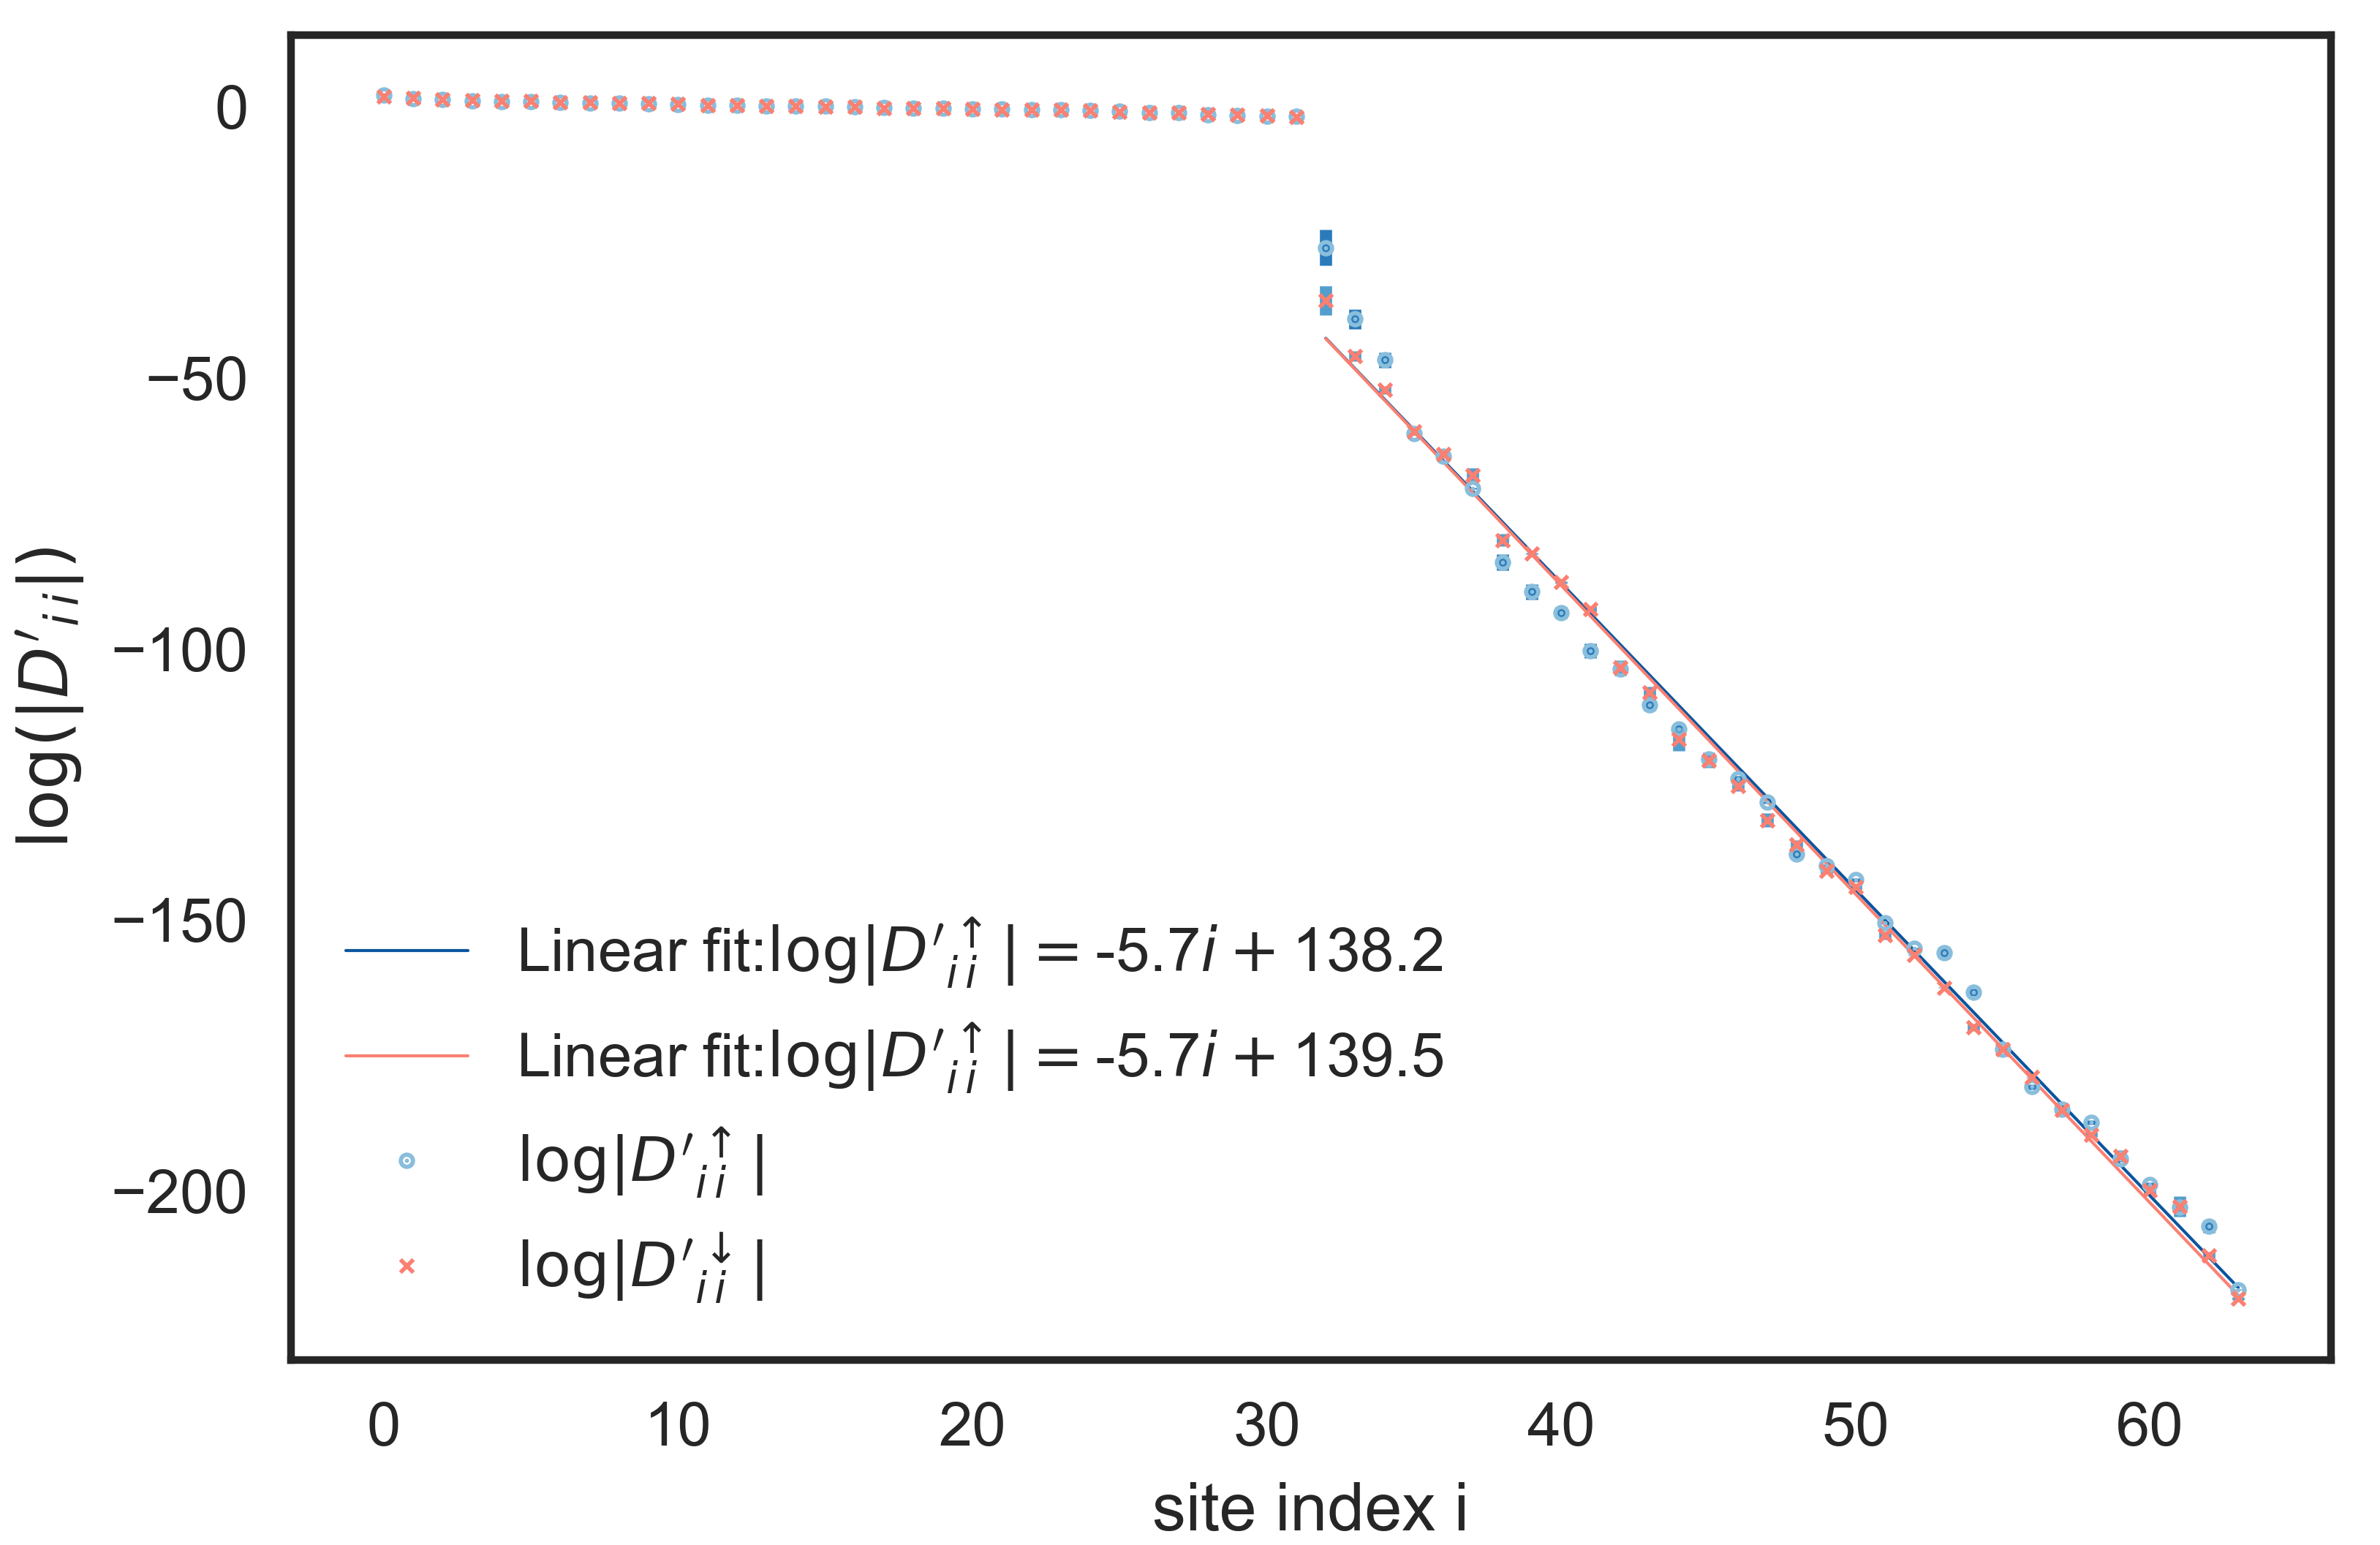
\includegraphics[scale=0.55]{Afqmc/OrdersOfMagnitude_N=64sites.png}
\hspace{0.3cm}
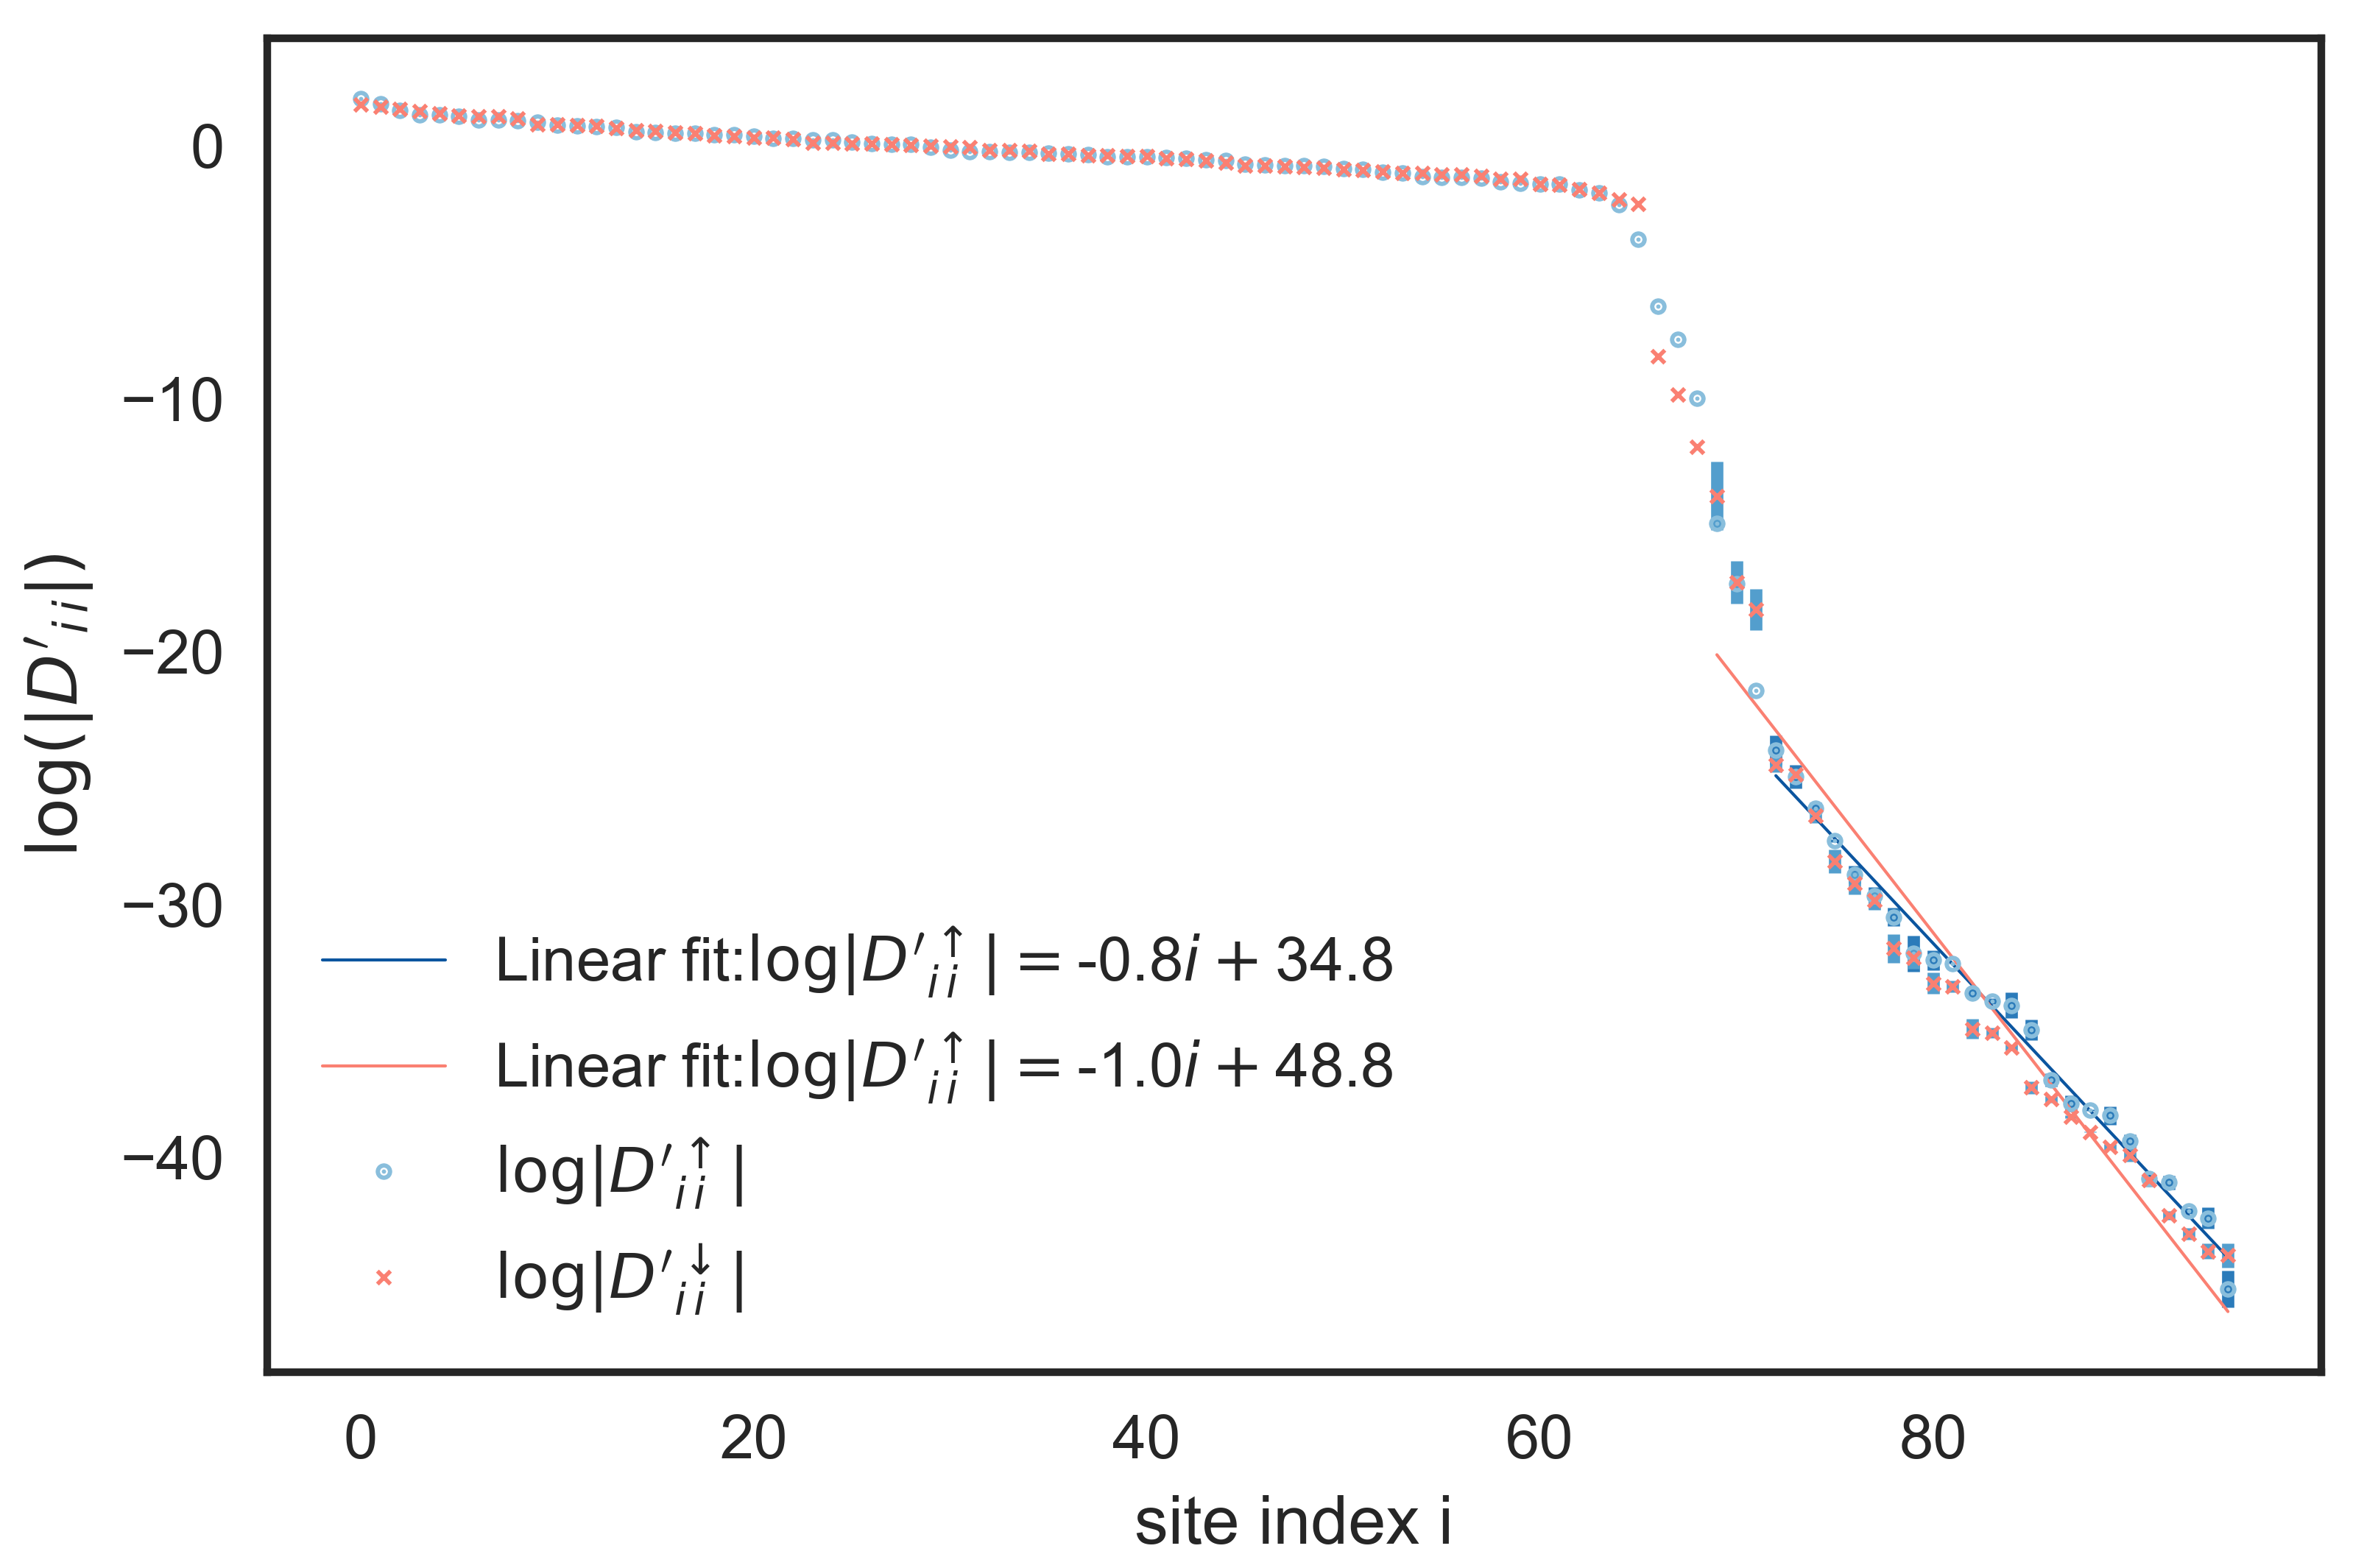
\includegraphics[scale=0.55]{Afqmc/OrdersOfMagnitude_N=96sites.png}
\caption[Exponentially divergent diagonal entries of $\bm D'$, showing the orders of magnitude spanned by the matrix elements of the stabilized matrix product.]{Exponentially divergent (and order one)  diagonal entries of $\bm D'$, showing the orders of magnitude spanned by the matrix elements of the stabilized matrix product.
The depicted systems are the same of Fig.(3.1). }
\end{figure}

The idea is to isolate the divergent scales in $\bm D$ right up until they are combined with the order one elements of $\bm Q^T \bm T^{-1}$, which cut off the divergent scales.
This is analogous to what happens in the band picture, where the unit term cuts off divergent scales in $e^{\beta ( E - \mu )}$ when we compute the occupation of a state (which is an element of the Green's matrix).
Notice that while $\bm Q$ and $\bm T$ are well conditioned, $\kappa ( \bm Q^T \bm T^{-1} + \bm D )$ and $\kappa ( \bm I + \prod_l \bm B_l )$ are comparable, and the upper bound on the error in the matrix elements of the inverse $( \bm Q^T \bm T^{-1} + \bm D )^{-1}$ is proportional to the condition number, which can be huge, due to the divergent scales in $\bm D$.

Then, how does this procedure work?
We gave an intuitive picture which we now make mathematically precise.
One may safely assume that $\bm Q^T \bm T^{-1}$ has moderate magnitude and condition number, so that when we add the first many elements of the diagonal $\bm D$, which are typically huge, we end up with diagonally dominant matrix.
Its first many rows are essentially a diagonal matrix plus a zero block on the right.
The remaining rows determine the effective condition number, so that $\kappa ( \bm Q^T \bm T^{-1} + \bm D )$ is actually reduced and the matrix becomes better conditioned.
This corresponds to defining numerical stability operationally.
We maintain the numerical scales explicitly, so that the information that we lose at the end is practically irrelevant in computing the Green's function: because of the way we organized the calculation, the overwriting of small scales by unit numbers and of unit scales by big numbers does not decrease precision, instead cutting off certain well picked numerical scales.
\begin{figure}[H]\label{fig:divergences}
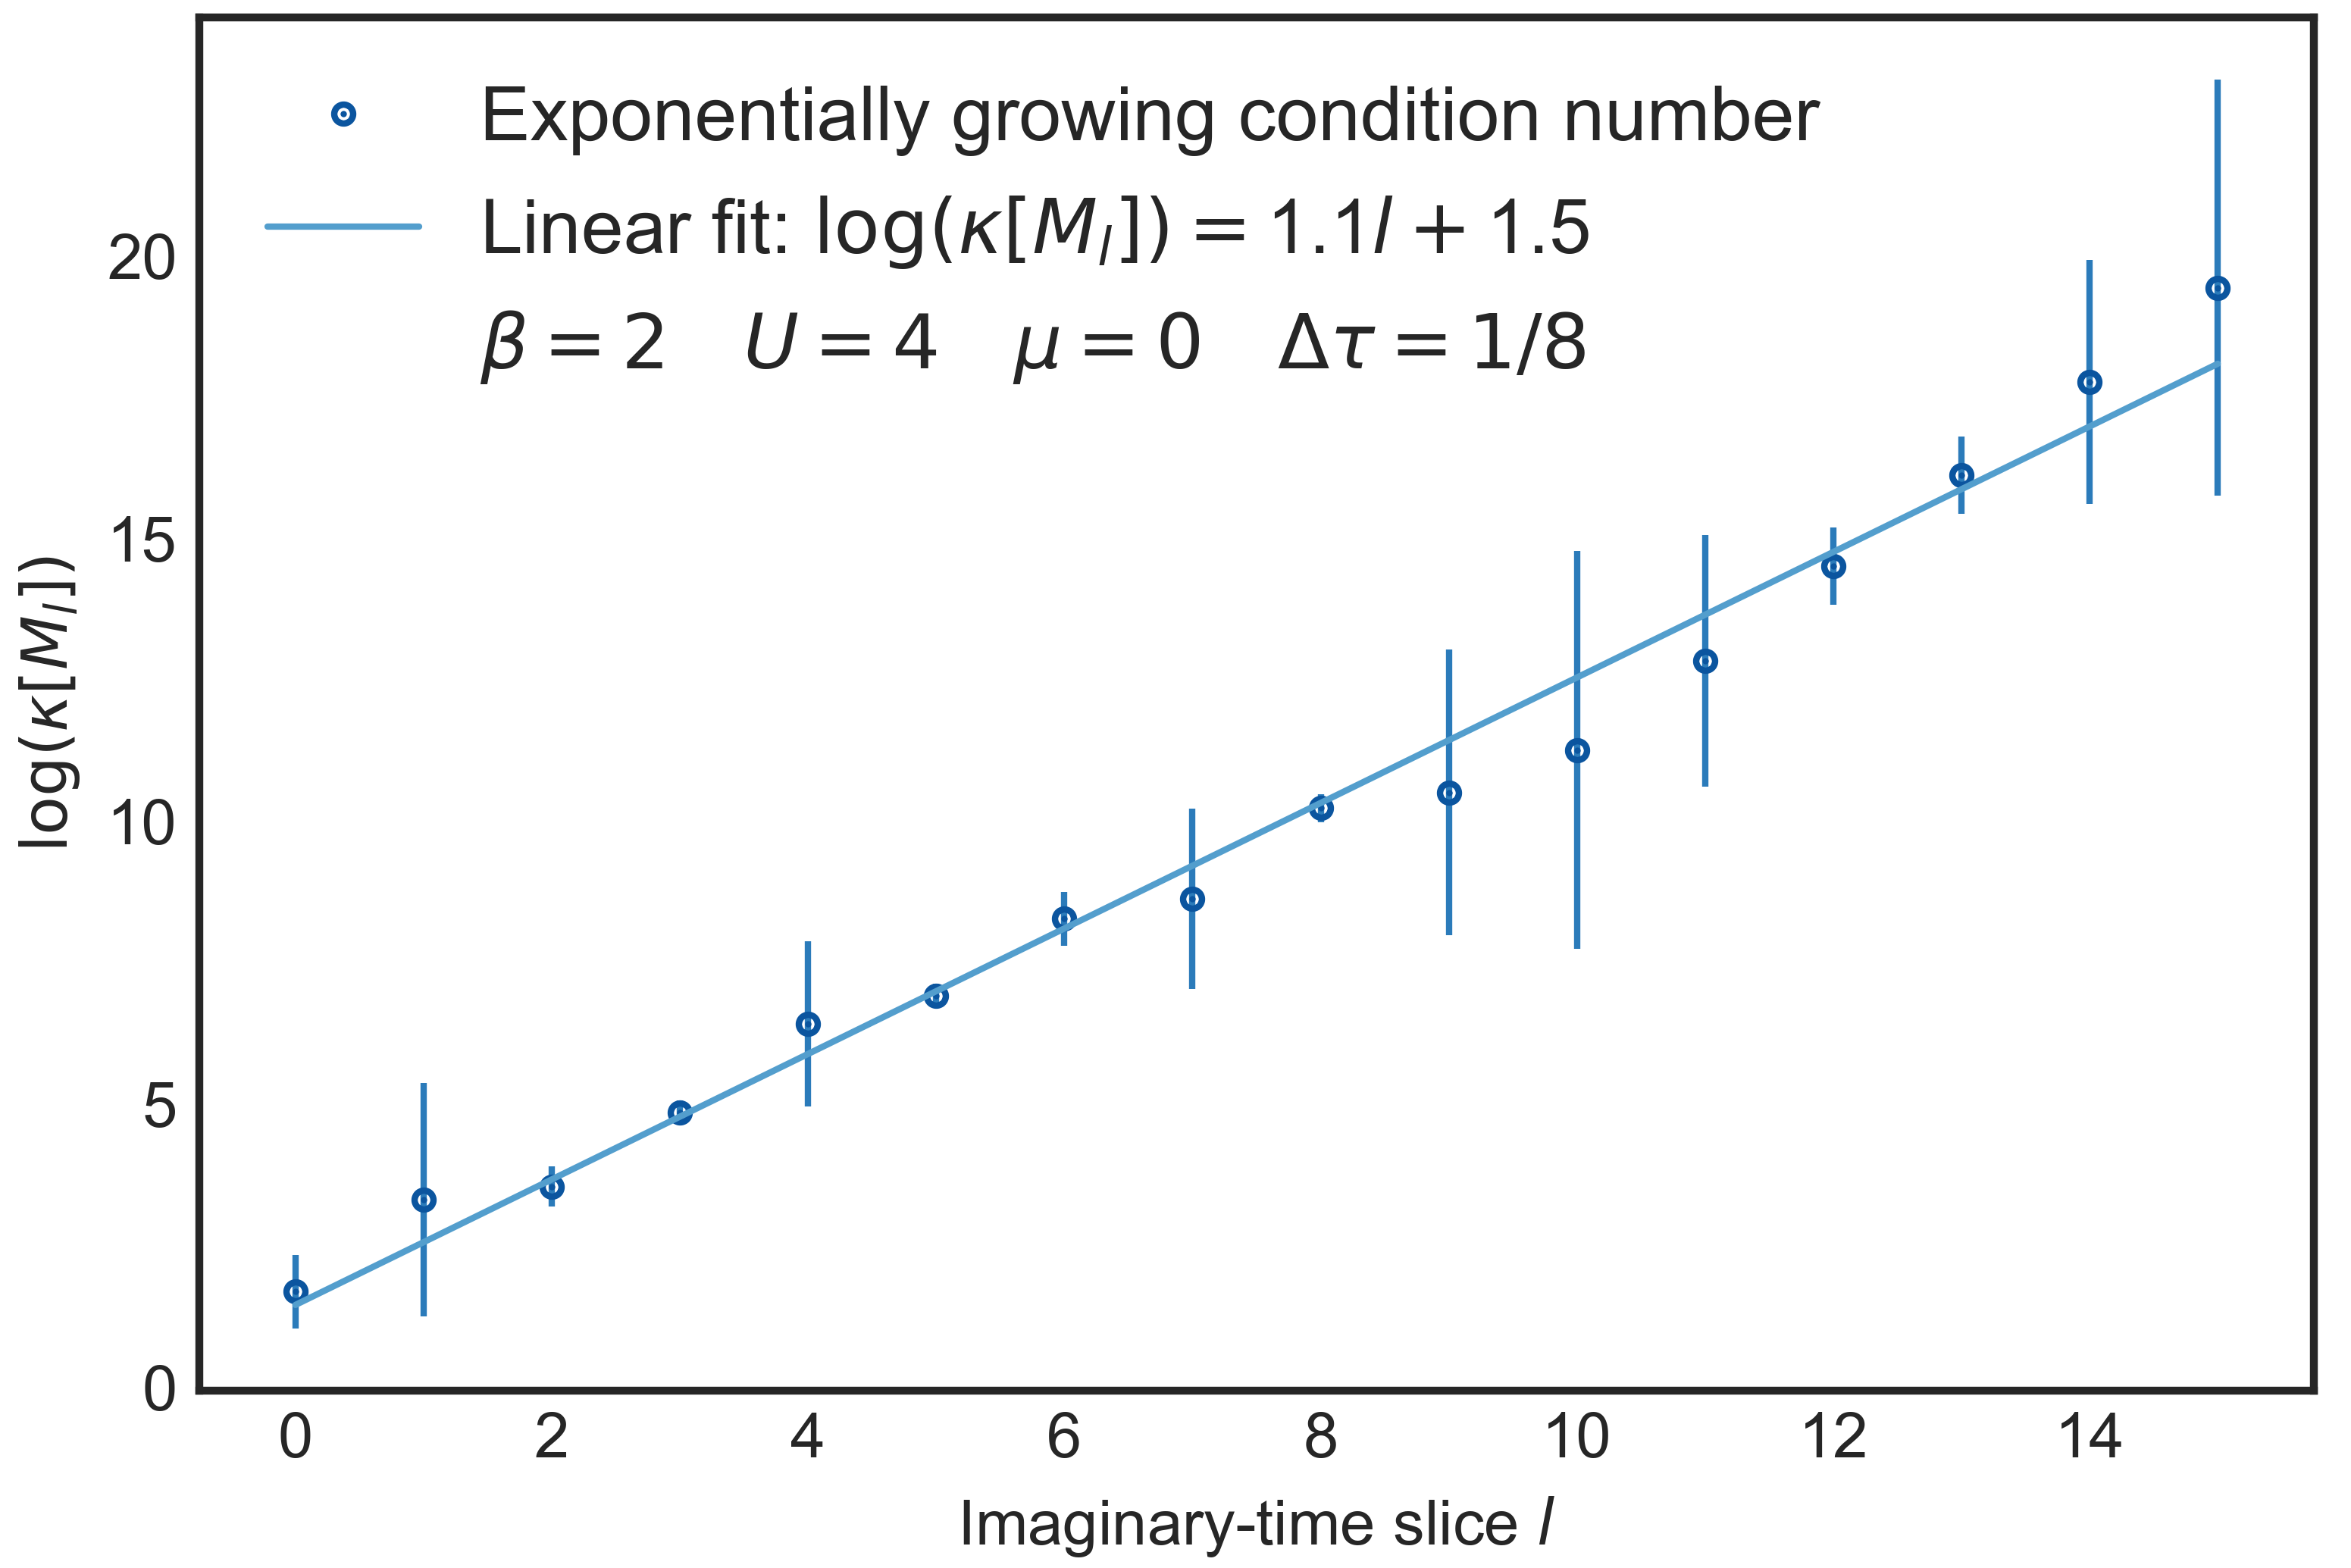
\includegraphics[scale=0.55]{Afqmc/conditionNumberNaive.png}
\hspace{-0.8cm}
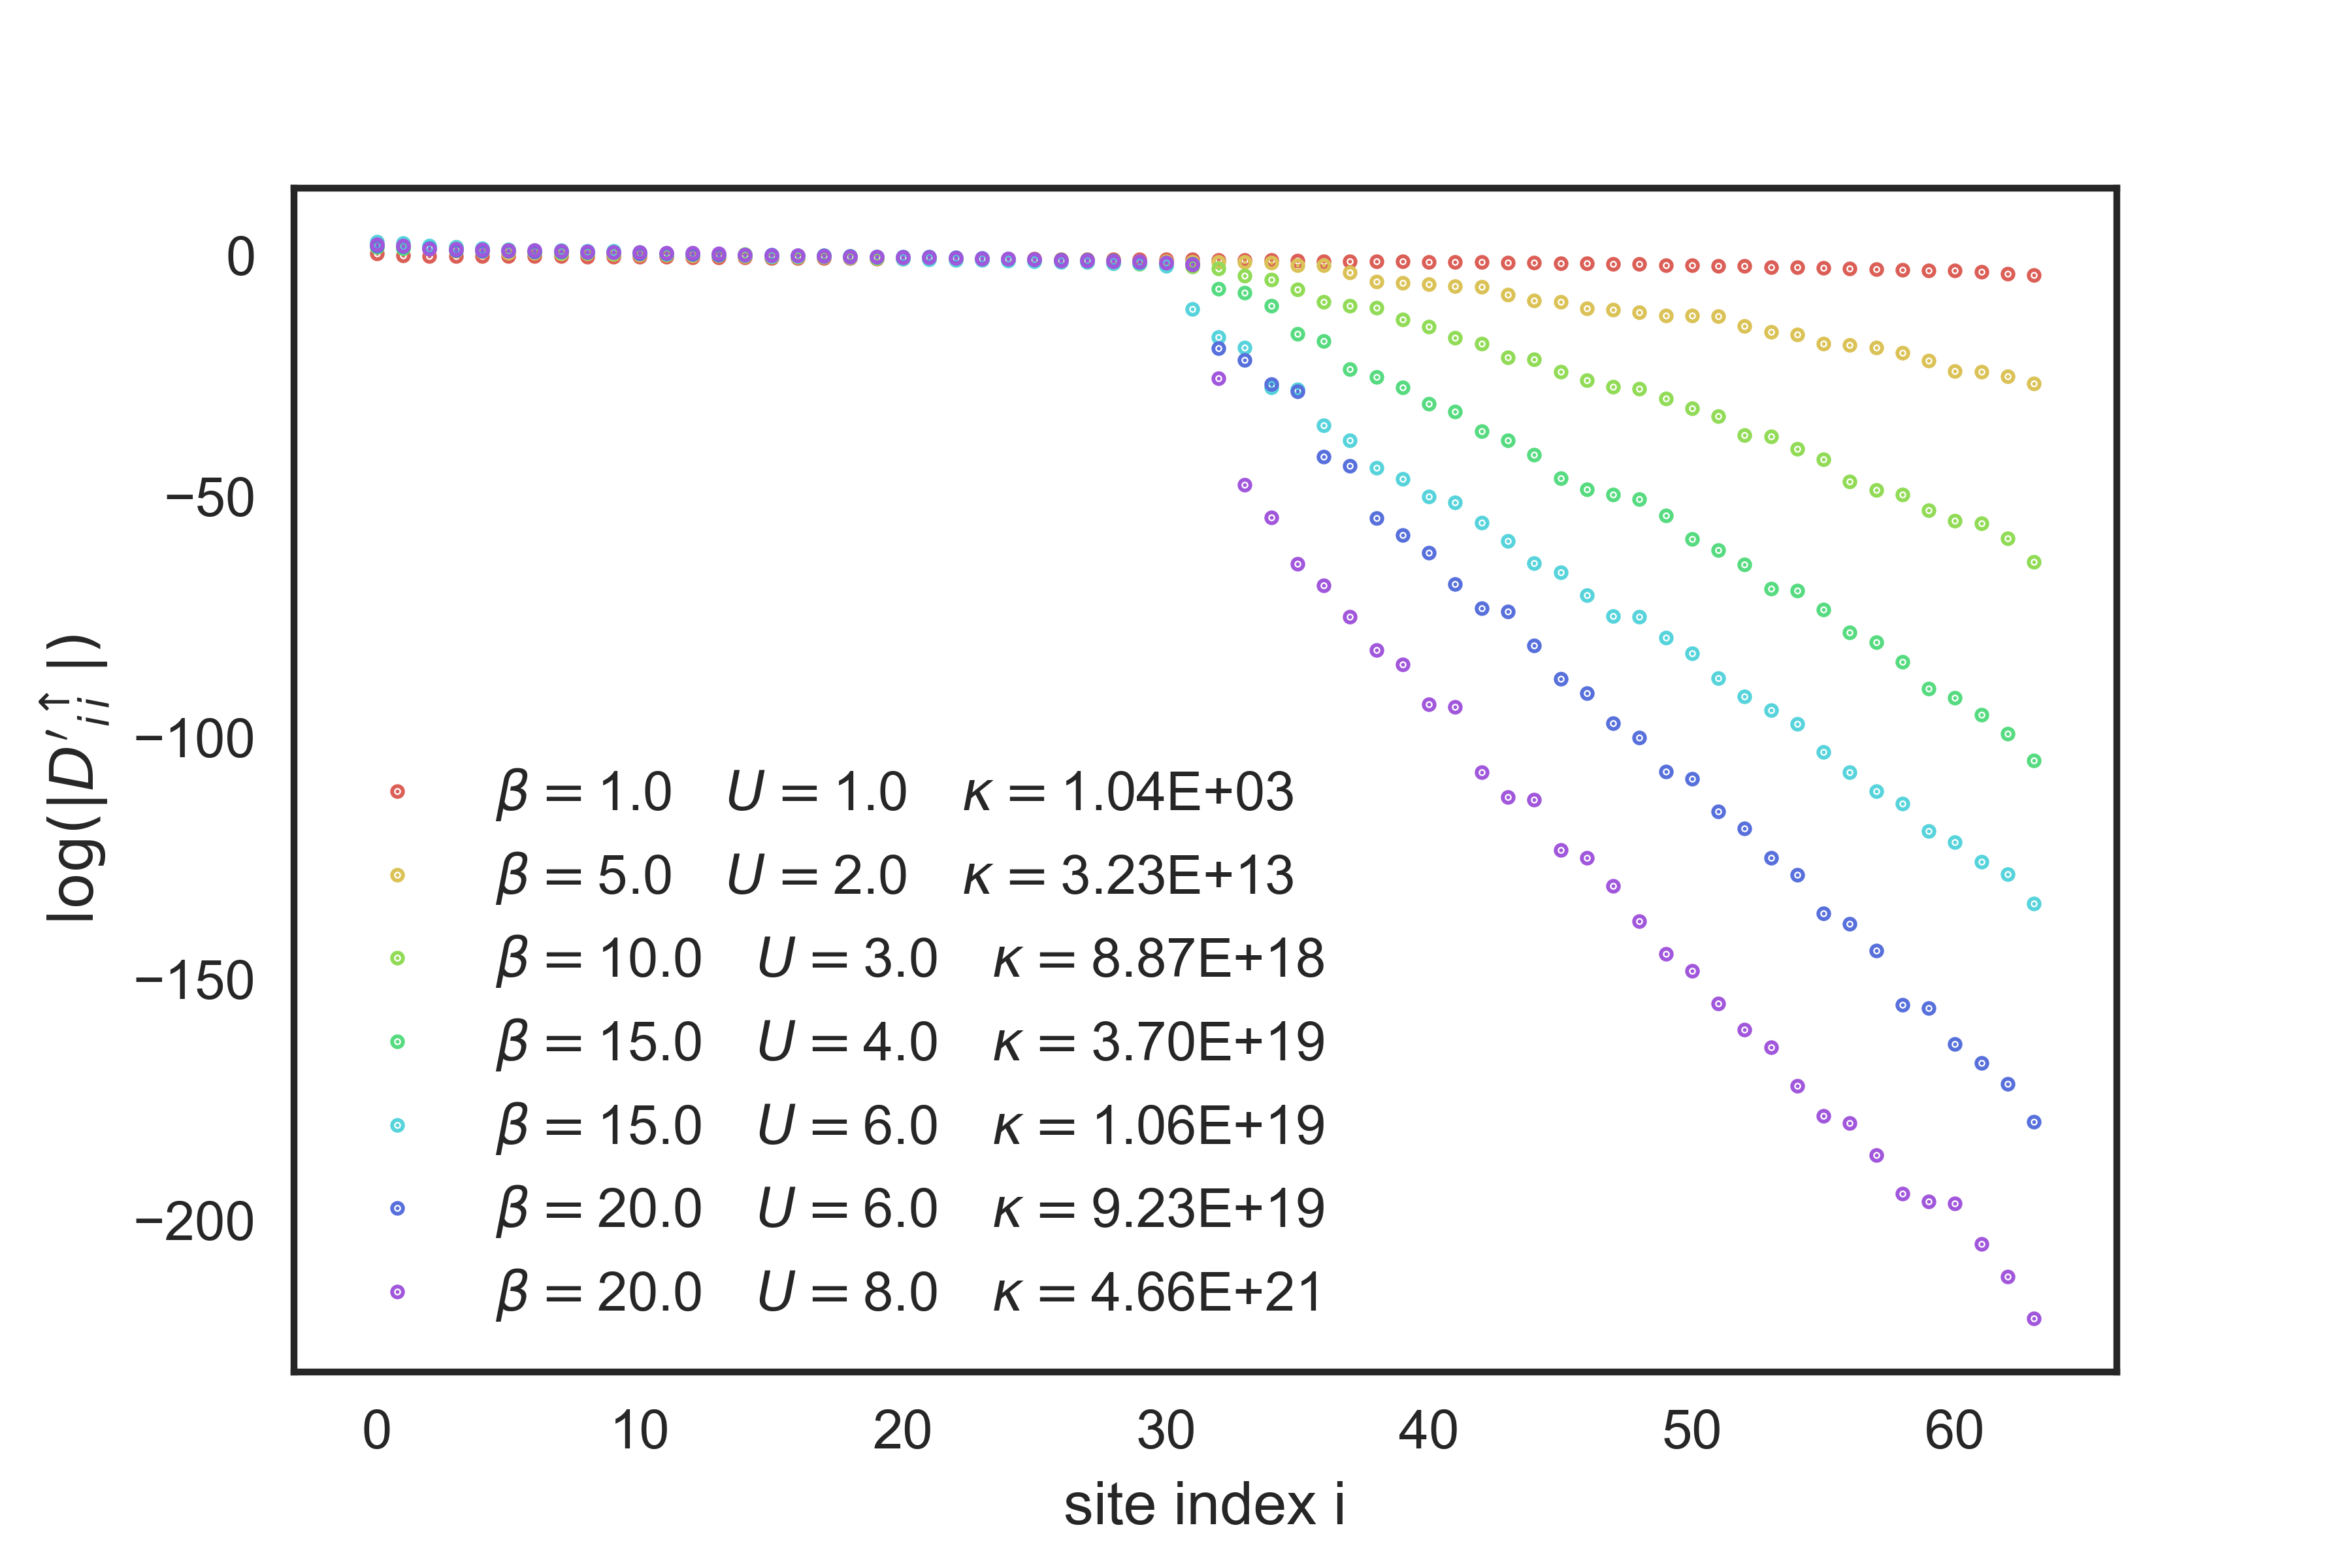
\includegraphics[scale=0.55]{Afqmc/DivergentScalesComparison.png}
\caption[Condition number of $\bm M_l = \prod_l \bm B_l$ obtained by multiplying $\bm B$-matrices naively. Absolute values of the diagonal entries of $\bm D'$ and corresponding condition number of the matrix to invert to obtain the Green's function.]{Left: Exponentially growing condition number $\kappa [ \bm M_l ]$ obtained by multiplying $\bm B$-matrices naively.
Right: Absolute values of the diagonal entries of $\bm D'$ for varying $\beta$ and $U$ and corresponding condition number of the matrix to invert to obtain the Green's function: $\kappa ( \bm Q^T \bm T^{-1} + \bm D )$.
Here, we show that are able to stabilize a multiplication of $\bm B$-matrices with elements spanning about 150 orders of magnitude, as can be seen by the elements of $\bm D'$. }
\end{figure}

In the band picture, our reasoning becomes particularly evident.
As long as a state deep into the band is occupied, it does not matter whether it is amplified by say $10^{100}$ or even $10^{1000}$.
The same applies for high energy states, which must be cut off anyway, so there is no problem in attenuating them by $10^{-100}$ or $10^{-1000}$.
In our calculation of $\bm G$, this corresponds to finding the single-particle states for fixed HS field $\bm h$ via the transformation matrices $\bm Q$ and $\bm T$.
The energy scales are stored in $\bm D$, so that when we add $\bm Q^T \bm T^{-1}$, the divergent scales are cut off, and so we can identify which states were amplified or attenuated.
These do not impact the calculation of $\bm G$ significantly, and because the computer cannot store big or small numbers anyway, it suffices to identify the big and small scales, which turn out not to contribute very much to $\bm G$.

A more accurate alternative proposed in \cite{bai_stable_2011} uses another more efficient method of separating the numerical scales.
The idea is to define two diagonal matrices of big and small entries, respectively $\bm D^b$ and $\bm D^s$, defined as
\begin{equation}
i = 0,..., N-1 :\,\,
D_{i i}^b =
\begin{cases}
D_{i i} , \,\, \text{if} \,\, | D_{i, i} | > 1 \\
1 , \,\, \text{otherwise}
\end{cases}
\quad
D_{i i}^s =
\begin{cases}
D_{i i} , \,\, \text{if} \,\, | D_{i, i} | \le 1 \\
1 , \,\, \text{otherwise}
\end{cases}
\end{equation}
so that $\bm D = \bm D^b \bm D^s$ .
Now, to compute the inverse, we can pull out $\bm D^b$, so that $(\bm D^b)^{-1}$ annihilates the top many rows of $\bm Q^T$, while $\bm D^s$ annihilates the bottom many rows of $\bm T$, isolating the relevant numerical scales, and leaving us with the fairly well conditioned matrix $(\bm D^b)^{-1} \bm Q^T + \bm D^s \bm T$ to invert.
\begin{equation}
( \bm Q^T \bm T^{-1} + \bm D^b \bm D^s )^{-1} = \bm T^{-1} [ (\bm D^b)^{-1} \bm Q^T + \bm D^s \bm T ]^{-1} (\bm D^b)^{-1}
\end{equation}

The matrix elements of $\bm G$ are computed accurately via the update scheme of Eq.(\ref{eq:updates}), however we can only use the wrapping of Eq.(\ref{eq:wrap}) (which effectively involves multiplying $\bm B$-matrices) to  \say{propagate} $\bm G$ for $L / \Lambda$ slices, after which $\bm G$ must be recomputed from scratch using the $\bm Q \bm D \bm T$ decompositions.
Thus, the cost of the stabilization is $\mathcal{O} ( \Lambda^2 ) \propto 
\beta^2$, which may dominate at very low temperatures for certain problems.
There is a great deal of recomputation involved in the stabilization, and we will present a method of storing the decomposition of the partial product of $\bm B$-matrices, so that the cost is reduced to $\mathcal{O}(\Lambda) \propto \beta$.
In practice, it is verified that sufficiently low temperatures to study say the ground state of the Hubbard model in the square lattice can be achieved with the stabilization overhead representing only a fraction of the simulation time \cite{hanke_electronic_nodate,white_numerical_1989}.

\subsection{Storing partial products and time-displaced Green's function}
\label{subsec:partial}

Given the $\bm Q \bm R \bm P$ decomposition of a matrix, we can obtain its $\bm P \bm R \bm Q$ decomposition (with partial pivoting), so that the partial products can be built up from the left through successive $\bm T_L \bm D_L \bm Q_L$ decompositions (the subscript meaning \say{left}).
Define the row/column reversing matrix 
\begin{equation}
\bm P_r \equiv
\begin{pmatrix}
 & & 1 \\
 & \rddots & \\
1& & 
\end{pmatrix}
\,\, \text{with} \,\, \bm P_r^T = \bm P_r \,\, \text{and} \,\, \bm P_r^{-1} = \bm P_r^T ,
\end{equation}
so that $\bm B \bm P_r$ reverses the order of the columns of $\bm B$, and $\bm P_r \bm B$ reverses the order of the rows.
Now $\bm Q \bm R \bm P$-decompose $(\bm P_r \bm B)^T = \tilde{\bm Q} \tilde{\bm R} \tilde{\bm P}$, and define $\bm Q \equiv \bm P_r \tilde{\bm Q}^T$, $\bm R \equiv \bm P_r \tilde{\bm R}^T \bm P_r$, $\bm P \equiv \bm P_r \tilde{\bm P}^T \bm P_r$, giving
\begin{equation}
\bm B = \underbrace{\bm P_r \bm P_r}_{\bm I} \bm B = \bm P_r ( \tilde{\bm Q} \tilde{\bm R} \tilde{\bm P} )^T =  \bm P_r \tilde{\bm P}^T \underbrace{\bm P_r \bm P_r}_{\bm I} \tilde{\bm R}^T \underbrace{\bm P_r \bm P_r}_{\bm I} \tilde{\bm Q}^T = \bm P \bm R \bm Q = \bm P \bm R \bm D^{-1} \bm D \bm Q \equiv \bm T \bm D \bm Q ,
\end{equation}
where we reversed the definition of $\bm T$, and the successive decompositions are obtained by multiplying other $\bm B$-matrices on the the right: $\bm T (\bm D \bm Q \bm B') = \bm T \bm T' \bm D' \bm Q'$, and so on.
At the first slice, we compute the partial products and store their decompositions
\begin{equation}
\underbrace{ \overbrace{ \underbrace{\bm B_{L - 1} \bm B_{L-2} ... \bm B_{L - 1- L / \Lambda}}_{(\bm T_L \bm D_L \bm Q_L)_{0} }  \bm B_{L - 2 - L / \Lambda} ...\bm B_{L - 2 - 2 L / \Lambda} }^{(\bm T_L \bm D_L \bm Q_L)_{1}} ... \bm B_{L / \Lambda - 1} ...  \bm B_0}_{(\bm T_L \bm D_L \bm Q_L)_{\Lambda - 1}}
\end{equation}
and as the $\bm B$-matrices are moved onto the left, we build their partial product from the right and decompose it in $\bm Q_R \bm D_R \bm T_R$, saving the resulting successive decompositions in place of the $\bm T_L \bm D_L \bm Q_L$ decompositions which become unneeded.
For example, when the second partial product is on the left:
\begin{equation}
\underbrace{\bm B_{L / \Lambda - 1} ...  \bm B_0}_{(\bm Q_R \bm D_R \bm T_R)_{0}} ... \overbrace{ \underbrace{\bm B_{L - 1} \bm B_{L-2} ... \bm B_{L - 1- L / \Lambda}}_{(\bm T_L \bm D_L \bm Q_L)_{0} } ...  \bm B_{2 L / \Lambda -1} ...\bm B_{L / \Lambda} }^{(\bm T_L \bm D_L \bm Q_L)_{\Lambda - 2}} 
\end{equation}
so that at the $\lambda$-th partial product, we obtain $(\bm Q_R \bm D_R \bm T_R )_{\lambda -1} (\bm T_L \bm D_L \bm Q_L )_{\Lambda - 1 - \lambda}$, and generally:
\begin{equation}
\bm G ( \tau, \tau ) = [\bm I + \bm B ( \tau, 0 ) \bm B ( \beta, \tau ) ]^{-1} = ( \bm I + \bm Q_R \bm D_R \bm T_R \bm T_L \bm D_L \bm Q_L )^{-1} = \bm Q_L^T ( \underbrace{\bm Q_R^T \bm Q_L^T + \bm D_R \bm T_R \bm T_L \bm D_L}_{\bm Q' \bm D' \bm T'} )^{-1} \bm Q_R^T ,
\end{equation}
where we may now apply any of the two methods described in the previous section to stably compute the inverse in brackets.
We will generalize the \say{cut off} method so as to obtain time-displaced Green's functions, the price to pay being that the matrices increase their size to $2 N \times 2 N$.

The inverse of a matrix composed of blocks is given by the Aitken block diagonalization formula
\begin{equation}
\begin{pmatrix}
\bm A & \bm B \\
\bm C & \bm D
\end{pmatrix}^{-1}
=
\begin{pmatrix}
( \bm A - \bm B \bm D^{-1} \bm C )^{-1} & ( \bm C - \bm D \bm B^{-1} \bm A )^{-1} \\
( \bm B - \bm A \bm C^{-1} \bm D )^{-1} & ( \bm D - \bm C \bm A^{-1} \bm B )^{-1}
\end{pmatrix}
\end{equation}

A particular choice of these matrices gives both the equal- and the unequal-time Green's functions:
\begin{equation}
\begin{pmatrix}
\bm I & \bm B_{\bm h} (\tau, 0) \\
-\bm B_{\bm h} ( \beta, \tau ) & \bm I
\end{pmatrix}^{-1}
=
\begin{pmatrix}
\bm G ( 0 ) & - ( \bm I - \bm G ( 0 ) ) \bm B_{\bm h} ( \tau, 0 )  \\
\bm B_{\bm h} ( \tau, 0 ) \bm G ( 0 ) & \bm G ( \tau ) 
\end{pmatrix}
=
\begin{pmatrix}
\bm G ( 0 ) & \bm G ( 0, \tau )  \\
\bm G ( \tau, 0 ) & \bm G ( \tau ) 
\end{pmatrix}
\end{equation}

We can now substitute the decompositions of the partial products that we store and update throughout the algorithm, and invert while being careful in isolating the diverging scales.
The method is very stable, but numerically more expensive since the matrices at hand are twice as big.
\begin{equation}
\begin{split}
\begin{pmatrix}
\bm I & \bm T_L \bm D_L \bm Q_L \\
\bm Q_R \bm D_R \bm T_R & \bm I
\end{pmatrix}^{-1}
&= \left[
\begin{pmatrix}
\bm T_L & 0 \\
0 & \bm Q_R 
\end{pmatrix}
\underbrace{\begin{pmatrix}
(\bm T_R \bm T_L)^{-1} & \bm D_L \\
- \bm D_R & (\bm Q_L \bm Q_R)^{-1}
\end{pmatrix}}_{\bm Q \bm D \bm T}
\begin{pmatrix}
\bm T_R & 0 \\
0 & \bm Q_L
\end{pmatrix}
\right]^{-1} \\
&= \left[
\begin{pmatrix}
\bm T_R^{-1} & 0 \\
0 & \bm Q_L^T
\end{pmatrix}
\bm T^{-1} \right]
\bm D^{-1}
\left[
\bm Q^T
\begin{pmatrix}
\bm T_L^{-1} & 0 \\
0 & \bm Q_R^T
\end{pmatrix}
\right]
\end{split}
\end{equation}
Here, $\bm D$ contains only large scales because the matrices with order one elements, $(\bm T_R \bm T_L)^{-1}$ and $(\bm Q_L \bm Q_R)^T$, cut off the exponentially small scales in $\bm D_L$ and $\bm D_R$.

This procedure of storing the decompositions of partial products is not only more efficient.
It also allows us to compute any observable, whether it requires equal or unequal time Green's functions, while still preserving the $\mathcal{O} (\beta N^3 )$ complexity of the algorithm.